% Tikz cơ bản 
% Mặt phẳng tọa độ Oxy
\begin{tikzpicture}[scale=0.8,>=stealth, font=\footnotesize, line join=round, line cap=round]
	\draw[color=gray!50,dashed] (-6,-6) grid (6,6);
	\draw[->] (-6,0)--(6,0) node [below]{$x$};
	\draw[->] (0,-6)--(0,6) node [left]{$y$};
	\clip (-6,-6) rectangle (6,6);
	%%%%%%%%%%%%%%%
	\tkzDefPoints{0/0/A,5/0/B}
	\tkzDrawPoints[fill=black,size=3](A,B,C)
	
\end{tikzpicture}

% Vẽ Điểm 
\tkzDrawPoints[fill=black,size=3](A,B,C)

% Vẽ đoạn 
\tkzDrawSegments(A,B B,C)

% Vẽ đường thẳng 
\tkzDrawLines[add=1cm and 1cm](A,B)

% Vẽ Vector
\tkzDrawVectors(A,B)

% Nhãn điểm 
\tkzLabelPoints[below](A)

% Nhãn Đoạn 
\tkzLabelSegment(A,B){$a$}

% Đa giác 
\tkzDrawPolygon(A,B,C)

% định nghĩa biến 
\def \x{2.5} 

% Vùng {scope} 
\begin{scope}
	
\end{scope}

% Định nghĩa điểm 
\tkzDefPoints{0/0/A,5/0/B}

% Tịnh tiến
\tkzDefPointBy[translation=from A to B](M)\tkzGetPoint{M'}

% Đối xứng trục
\tkzDefPointBy[reflection=over A--B](M)\tkzGetPoint{M'}

% Đối xứng tâm 
\coordinate (M') at ($(I)!-1!(M)$);

% Phép quay
\tkzDefPointBy[rotation=center I angle 45](M)\tkzGetPoint{M'}

% Phép vị tự 
\coordinate (M') at ($(I)!k!(M)$);

% Chiếu vuông góc 
\tkzDefPointBy[projection=onto A--B](M)\tkzGetPoint{M'}

% Trung điểm 
\coordinate (I) at ($(A)!0.5!(B)$);

% Trọng Tâm 
\tkzCentroid(A,B,C)\tkzGetPoint{G}

% Tâm đường tròn ngoại tiếp tam giác 
\tkzCircumCenter(A,B,C)\tkzGetPoint{I}

% Tâm đường tròn nội tiếp tam giác  
\tkzInCenter(A,B,C)\tkzGetPoint{I}

% C để tam giác ABC đều 
\tkzDefEquilateral(A,B)\tkzGetPoint{C}

% C, D để ABCD là hình vuông 
\tkzDefSquare(A,B)\tkzGetPoints{C}{D}

% C cho góc A, B
\tkzDefTriangle[two angles=30 and 45](A,B)\tkzGetPoint{C}

% Giao điểm của AB và CD 
\tkzInterLL(A,B)(C,D)\tkzGetPoint{I}

% Giao AB với đường tròn (I,M) 
\tkzInterLC(A,B)(I,M)\tkzGetPoints{C}{D}

% Giao AB với đường tròn tâm I, bán kính bằng 2 
\tkzInterLC[R](A,B)(I,2cm)\tkzGetPoints{C}{D}

% Giao 2 đường tròn 
\tkzInterCC(I,A)(J,B)\tkzGetPoints{C}{D}

% Giao 2 đường tròn có bán kính 2, 3 cm 
\tkzInterCC[R](I,2cm)(J,3cm)\tkzGetPoints{C}{D}

% Điểm trên đường tròn (I, 3)
\coordinate (M) at ($(I)+(60:3cm)$);

% Điểm trên Elip
\coordinate (M) at ($(I)+(60:3cm and 2cm)$);

% Vẽ các nét thẳng: 

% Đường cao tam giác từ A
\tkzDrawAltitude(B,C)(A)

% Đường trung tuyến từ A 
\tkzDrawMedian(B,C)(A)

% Đường phân giác từ A 
\tkzDrawBisector(B,A,C)\tkzGetPoint{A'}

% d qua C, song song với AB 
\tkzDefLine[parallel=through C](A,B) \tkzGetPoint{d}

% d qua C, vuông góc với AB  
\tkzDefLine[orthogonal=through C](A,B)\tkzGetPoint{d}

% Vẽ các nét cong 

% Vẽ đường tròn tâm I, bán kính IA  
\tkzDrawCircle[radius](I,A)

% đường tròn tâm I, bán kính bằng 2 
\draw (I) circle(2cm);

% đường tròn đường kính AB  
\tkzDrawCircle[diameter](A,B)

% đường tròn đi qua 3 điểm  
\tkzDrawCircle[circum](A,B,C)

% đường tròn nội tiếp tam giác 
\tkzDrawCircle[in](A,B,C)

% Cung tâm I, từ A, góc 60 
\tkzDrawArc[color=black,thin,rotate](I,A)(60)

% cung tâm I, bán kính 2 cm từ 30 đến 75  
\tkzDrawArc[R](I,2cm)(30,75)

% Ellipse tâm I có bán kính 3 cm và 1.6 cm 
\draw (I) ellipse (3cm and 1.6cm);

% Cung Ellipse từ a đến b
\draw (A) arc (0:120:3cm and 1.6cm);

% Đường cong controls
\draw (A)..controls (x1,y1) and (x1,y1)..(B);

% Đường cong qua n điểm  
\draw plot[smooth,tension=0.65] coordinates{(x1,y1) (x2,y2) (xn,yn)};

% Parabola bend 
\draw (x1,y1) parabola bend (x2,y2) (x3,y3);

% Biểu đồ venn  
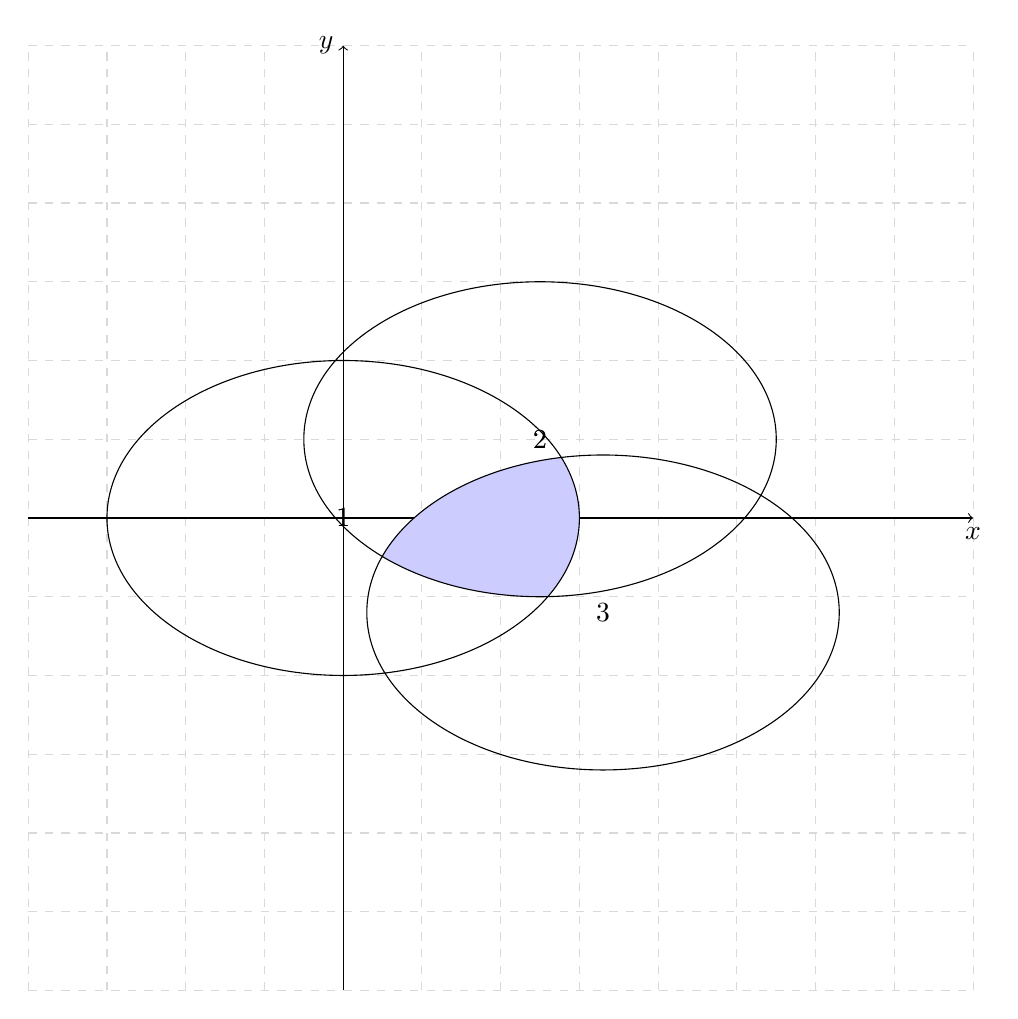
\begin{tikzpicture}[scale=1]
	\draw[color=gray!30,dashed] (-4,-6) grid (8,6);
	\draw[->] (-4,0)--(8,0) node [below]{$x$};
	\draw[->] (0,-6)--(0,6) node [left]{$y$};
	\clip (-4,-6) rectangle (8,6);
	%%%%%%%%
	\def\firstven{(0,0) ellipse (3cm and 2cm) node{1}}
	\def\secondven{(2.5,1) ellipse (3cm and 2cm) node{2}}
	\def\thirdven{(3.3,-1.2) ellipse (3cm and 2cm) node{3}}
	\begin{scope}
		\clip \firstven;
		\clip \secondven;
		\fill[blue!20] \thirdven;
	\end{scope}
	\draw \firstven \secondven \thirdven;
\end{tikzpicture}

% Đánh dấu, tô nền 

% Đánh dấu đoạn 
\tkzMarkSegments[mark=||](A,B A,C)

% đánh dấu góc vuông 
\tkzMarkRightAngles[size=0.17](A,B,C)

% Đánh dấu góc tròn  
\tkzMarkAngles[size=0.7cm,arc=ll,mark=|](A,B,C)

% Gắn nhãn cho góc 
\tkzLabelAngles[pos=1,rotate=30](A,B,C){$\alpha$}

% Tô nền đa giác 
\tkzFillPolygon[color=green!80, fill opacity=0.5](A,B,C)

% Tô miền tích phân 
\fill[pattern=north east lines,opacity=0.8] plot[domain=-1:3](\x,{(\x)^3-3*(\x)^2-\x+3})--cycle;

% Biểu diễn cung lượng giác 
\begin{tikzpicture}[scale=2, line width=1pt]
	\fill (0,0) circle (0.3pt) node[below right]{$O$};
	\fill (1,0) circle (0.3pt) node[above right]{$1$};
	\fill (-1,0) circle (0.3pt) node[above left]{$-1$};
	\fill (0,1) circle (0.3pt) node[above right]{$1$};
	\fill (0,-1) circle (0.3pt) node[below left]{$-1$};
	\trucLG%Hệ trục
	%$x=\dfrac{\pi}{6}+k\dfrac{2\pi}{5}$
	\pointLG{30}{5}{*}{red}	
	pointLG{<góc>}{<n>}{<nhãn>}{<màu>}
	%$x=\dfrac{\pi}{4}+k\pi$
	\pointLG{45}{2}{star}{violet}
	%$x=\dfrac{5\pi}{6}+k\dfrac{\pi}{3}$
	\pointLG{150}{6}{triangle}{blue}
\end{tikzpicture}

% Vẽ hình không gian 

% Tứ diện cơ bản  
\begin{tikzpicture}[scale=1,>=stealth, font=\footnotesize, line join=round, line cap=round]
	\tkzDefPoints{0/0/B,1.3/-1.6/C,4.5/0/D,1/3.5/A}
	\tkzDrawPolygon(A,B,C,D)
	\tkzDrawSegments(A,C)
	\tkzDrawSegments[dashed](B,D)
	\tkzDrawPoints[fill=black,size=4](A,B,C,D)
	\tkzLabelPoints[above](A)
	\tkzLabelPoints[below](C)
	\tkzLabelPoints[left](B)
	\tkzLabelPoints[right](D)
\end{tikzpicture}

% Hình chóp S.ABC có chiều cao h = SA 
\begin{tikzpicture}[scale=1,>=stealth, font=\footnotesize, line join=round, line cap=round]
	\tkzDefPoints{0/0/A,1.2/-1.5/B,4/0/C}
	\coordinate (S) at ($(A)+(0,3)$);
	\tkzDrawPolygon(S,A,B,C)
	\tkzDrawSegments(S,B)
	\tkzDrawSegments[dashed](A,C)
	\tkzDrawPoints[fill=black,size=4](A,B,C,S)
	\tkzMarkRightAngles[size=0.16](S,A,B S,A,C)
	\tkzLabelPoints[above](S)
	\tkzLabelPoints[below](B)
	\tkzLabelPoints[left](A)
	\tkzLabelPoints[right](C)
\end{tikzpicture}

% Hình chóp tam giác đều S.ABC  
\begin{tikzpicture}[scale=1,>=stealth, font=\footnotesize, line join=round, line cap=round]
	\tkzDefPoints{0/0/A,1.2/-1.6/B,4.5/0/C}
	\tkzCentroid(A,B,C)\tkzGetPoint{G}
	\coordinate (S) at ($(G)+(0,3.5)$);
	\coordinate (M) at ($(B)!1/2!(C)$);
	\tkzDrawPolygon(A,B,C,S)
	\tkzDrawSegments(S,B)
	\tkzDrawSegments[dashed](M,A A,C S,G)
	\tkzDrawPoints[fill=black,size=4](A,B,C,S,G,M)
	\tkzMarkRightAngles[size=0.14](A,M,B S,G,A)
	\tkzLabelPoints[above](S)
	\tkzLabelPoints[below](B,G,M)
	\tkzLabelPoints[left](A)
	\tkzLabelPoints[right](C)
\end{tikzpicture}

% Hình chóp S.ABC có SBC là mặt đứng 
\begin{tikzpicture}[scale=1,>=stealth, font=\footnotesize, line join=round, line cap=round]
	\tkzDefPoints{0/0/B,1/-1.5/A,4/0/C}
	\coordinate (H) at ($(B)!0.5!(C)$);
	\coordinate (S) at ($(H)+(0,3)$);
	\tkzDrawPolygon(S,B,A,C)
	\tkzDrawSegments(S,A)
	\tkzDrawSegments[dashed](S,H)
	\tkzDrawSegments[dashed](B,C)
	\tkzDrawPoints[fill=black,size=4](A,B,C,S,H)
	\tkzLabelPoints[above](S)
	\tkzLabelPoints[below](H,A)
	\tkzLabelPoints[left](B)
	\tkzLabelPoints[right](C)
\end{tikzpicture}

% Hình chóp S.ABCD có chiều cao h = SA 
\begin{tikzpicture}[scale=1,>=stealth, font=\footnotesize, line join=round, line cap=round]
\tkzDefPoints{0/0/A,-1.3/-1.6/B,2.5/-1.6/C}
\coordinate (D) at ($(A)+(C)-(B)$);
\coordinate (S) at ($(A)+(0,3)$);
\tkzDrawPolygon(S,B,C,D)
\tkzDrawSegments(S,C)
\tkzDrawSegments[dashed](A,S A,B A,D)
\tkzDrawPoints[fill=black,size=4](D,C,A,B,S)
\tkzMarkRightAngles[size=0.16](S,A,B S,A,D)
\tkzLabelPoints[above](S)
\tkzLabelPoints[below](A,B,C)
\tkzLabelPoints[right](D)
\end{tikzpicture}

% Hình chóp tứ giác đều S.ABCD  
\begin{tikzpicture}[scale=1,>=stealth, font=\footnotesize, line join=round, line cap=round]
	\tkzDefPoints{0/0/A,-1.9/-1.6/B,1.6/-1.6/C}
	\coordinate (D) at ($(A)+(C)-(B)$);
	\coordinate (O) at ($(A)!1/2!(C)$);
	\coordinate (S) at ($(O)+(0,3.5)$);
	\tkzDrawPolygon(S,B,C,D)
	\tkzDrawSegments(S,C)
	\tkzDrawSegments[dashed](A,S A,B A,D A,C B,D S,O)
	\tkzDrawPoints[fill=black,size=4](D,C,A,B,S)
	\tkzMarkRightAngles[size=0.16](A,O,B S,O,A S,O,B)
	\tkzLabelPoints[above](S)
	\tkzLabelPoints[below](A,C,O))
	\tkzLabelPoints[below left](B)
	\tkzLabelPoints[right](D)
\end{tikzpicture}

% Hình chóp S.ABCD có mặt đứng SAB  
\begin{tikzpicture}[scale=1,>=stealth, font=\footnotesize, line join=round, line cap=round]
	\tkzDefPoints{0/0/A,-1.4/-1.6/B,2.5/-1.6/C}
	\coordinate (D) at ($(A)+(C)-(B)$);
	\coordinate (H) at ($(A)!1/2!(B)$);
	\coordinate (S) at ($(H)+(0,3.5)$);
	\tkzDrawPolygon(S,B,C,D)
	\tkzDrawSegments(S,C)
	\tkzDrawSegments[dashed](A,S A,B A,D S,H)
	\tkzDrawPoints[fill=black,size=4](D,C,A,B,S,H)
	\tkzLabelPoints[above](S)
	\tkzLabelPoints[below](A,B,C)
	\tkzLabelPoints[left](H)
	\tkzLabelPoints[right](D)
\end{tikzpicture}

% Lăng trụ đứng tam giác  
\begin{tikzpicture}[scale=1,>=stealth, font=\footnotesize, line join=round, line cap=round]
	\tkzDefPoints{0/0/A,1.1/-1.5/B,3.5/0/C}
	\coordinate (A') at ($(A)+(0,3.2)$);
	\tkzDefPointsBy[translation=from A to A'](B,C){B'}{C'}
	\tkzDrawPolygon(A,B,C,C',B',A')
	\tkzDrawSegments(A',C' B',B)
	\tkzDrawSegments[dashed](A,C)
	\tkzDrawPoints[fill=black,size=4](A,C,B,A',B',C')
	\tkzLabelPoints[above](B')
	\tkzLabelPoints[below](B)
	\tkzLabelPoints[left](A',A)
	\tkzLabelPoints[right](C',C)
\end{tikzpicture}

% Lăng trụ xiên tam giác  
\begin{tikzpicture}[scale=1,>=stealth, font=\footnotesize, line join=round, line cap=round]
	\tkzDefPoints{0/0/A,1.2/-1.5/B,3.5/0/C}
	\coordinate (H) at ($(A)!1/2!(B)$);
	\coordinate (A') at ($(H)+(0,4)$);
	\tkzDefPointsBy[translation = from A to A'](B,C){B'}{C'}
	\tkzDrawPolygon(A,B,C,C',B',A')
	\tkzDrawSegments(A',C' B',B A',H)
	\tkzDrawSegments[dashed](A,C)
	\tkzDrawPoints[fill=black,size=4](A,C,B,A',B',C')
	\tkzLabelPoints[above](B')
	\tkzLabelPoints[below](B)
	\tkzLabelPoints[left](A',A,H)
	\tkzLabelPoints[right](C',C)
\end{tikzpicture}

% Hình hộp chữ nhật  
\begin{tikzpicture}[scale=1,>=stealth, font=\footnotesize, line join=round, line cap=round]
	\tkzDefPoints{0/0/A,-1.3/-1.1/B,2/-1.1/C}
	\coordinate (D) at ($(A)+(C)-(B)$);
	\coordinate (A') at ($(A)+(0,2.5)$);
	\tkzDefPointsBy[translation=from A to A'](B,C,D){B'}{C'}{D'}
	\tkzDrawPolygon(A',B',B,C,D,D')
	\tkzDrawSegments(B',C' C',D' C,C')
	\tkzDrawSegments[dashed](A,B A,D A,A')
	\tkzDrawPoints[fill=black,size=4](A,B,D,C,A',B',C',D')
	\tkzLabelPoints[above](A',D')
	\tkzLabelPoints[below](A,B,C)
	\tkzLabelPoints[left](B')
	\tkzLabelPoints[right](C',D)
\end{tikzpicture}

% Hình nón cơ bản  
\begin{tikzpicture}[scale=1,>=stealth, font=\footnotesize, line join=round, line cap=round]
	\def \x{2.2} %bán kính trục lớn elip
	\def \y{0.9} %bán kính trục bé elip
	\def \h{3.5} %chiều cao hình nón
	\coordinate (O) at (0,0);
	\coordinate (S) at ($(O)+(0,\h)$);
	\coordinate (M) at (-60:\x cm and \y cm);
	\coordinate (N) at ($(O)!-1!(M)$);
	\coordinate (l) at (168:\x cm and \y cm);
	\coordinate (r) at (12:\x cm and \y cm);
	\draw[dashed] (r) arc (12:168:\x cm and \y cm);
	\draw (r) arc (12:-192:\x cm and \y cm);
	\tkzDrawSegments(S,l S,r S,M)
	\tkzDrawSegments[dashed](S,O M,N S,N)
	\tkzDrawPoints[fill=black,size=4](O,S,N)
	\tkzLabelPoints[above](S);
	\tkzLabelPoints[below](O,M,N);
	\tkzMarkRightAngles[size=0.14](S,O,M)
\end{tikzpicture}

% Vị trí tương đối của Mặt Cầu và Mặt Phẳng - Tiếp xúc 
\begin{tikzpicture}[scale=1,>=stealth, font=\footnotesize, line join=round, line cap=round]
	\def \x{2} %bán kính trục lớn elip
	\def \y{0.8} %bán kính trục bé elip
	\coordinate (I) at (0,0);
	\coordinate (B) at (\x,0);
	\coordinate (A) at (-\x,0);
	\coordinate (H) at (-90:\x);
	\coordinate (m) at ($(H)+(-\x-1,-\y)$);
	\coordinate (n) at ($(H)+(\x-0.2,-\y)$);
	\coordinate (p) at ($(H)+(\x+0.7,\y)$);
	\coordinate (q) at ($(m)+(p)-(n)$);
	\tkzDrawCircle[radius](I,A)
	\draw[dashed] (A)--(B) arc (0:180:\x cm and \y cm);
	\draw (B) arc (0:-180:\x cm and \y cm);
	\tkzInterLC(p,q)(I,A)\tkzGetPoints{p'}{q'}
	\tkzDrawSegments[dashed](p',q' I,H)
	\tkzDrawSegments(q',q q,m m,n n,p p,p')
	\tkzDrawPoints[fill=black,size=4](A,B,I,H)
	\tkzLabelPoints[left](A)
	\tkzLabelPoints[right](B)
	\tkzLabelPoints[above](I)
	\tkzLabelPoints[below](H)
	\tkzMarkAngles[size=0.6cm,arc=l](n,m,q)
	\tkzLabelAngles[pos=0.38](n,m,q){$\alpha$}
\end{tikzpicture}

% Vị trí tương đối của Mặt Cầu và Mặt Phẳng - Cắt nhau 
\begin{tikzpicture}[scale=1,>=stealth, font=\footnotesize, line join=round, line cap=round]
	\def \x{2} %bán kính trục lớn elip
	\def \y{0.7} %bán kính trục bé elip
	\coordinate (I) at (0,0);
	\coordinate (B) at (\x,0);
	\coordinate (A) at (-\x,0);
	\coordinate (H) at ($(0,-0.5*\x)+(0,0.05)$);
	\coordinate (M) at ($(H)+(-60:\x*0.866 cm and \y*0.866 cm)$);
	\coordinate (m) at ($(H)+(-\x-1.1,-\y)$);
	\coordinate (n) at ($(H)+(\x+0.1,-\y)$);
	\coordinate (p) at ($(H)+(\x+0.9,\y)$);
	\coordinate (q) at ($(m)+(p)-(n)$);
	\tkzInterLC(p,q)(I,A)\tkzGetPoints{p'}{q'}
	\tkzInterLC(m,n)(I,A)\tkzGetPoints{x}{y}
	\draw (-34:\x) arc (-34:214:\x);
	\draw (y) arc (-124:-56:\x);
	\draw (x)[dashed] arc (-56:-30:\x);
	\draw (y)[dashed] arc (-124:-150:\x);
	\draw[dashed] ($(-30:\x)+(0,0.05)$) arc (0:180:\x*0.866 cm and \y*0.866 cm);
	\draw ($(-30:\x)+(0,0.05)$) arc (0:-180:\x*0.866 cm and \y*0.866 cm);
	\draw[dashed] (p')--(q') (I)--(H) (I)--(M) (H)--(M);
	\tkzDrawSegments(q',q q,m m,n n,p p,p')
	\tkzDrawPoints[fill=black,size=4](I,H,M)
	\tkzLabelPoints[above](I)
	\tkzLabelPoints[left](H)
	\node at ($(M)+(0.2,0.25)$) {$M$};
	\tkzMarkAngles[size=0.6cm,arc=l](n,m,q)
	\tkzLabelAngles[pos=0.38](n,m,q){$\alpha$}
\end{tikzpicture}

% Hình cầu đơn giản  
\begin{tikzpicture}[scale=1, line join=round, line cap=round]
	\def \x{2} %bán kính trục lớn elip
	\def \y{0.8} %bán kính trục bé elip
	\coordinate (A) at (0,0);
	\coordinate (B) at (2*\x,0);
	\coordinate (O) at ($(A)!0.5!(B)$);
	\tkzDrawCircle[radius](O,B)
	\draw[dashed] (B) arc (0:180:\x cm and \y cm);
	\draw (B) arc (0:-180:\x cm and \y cm);
	\tkzDrawSegments[dashed](A,B)
	\tkzDrawPoints(A,B,O)
	\tkzLabelPoints[left](A)
	\tkzLabelPoints[right](B)
	\tkzLabelPoints[below](O)
\end{tikzpicture}

% Đồ thị hàm số 

% Hàm số bậc 2 
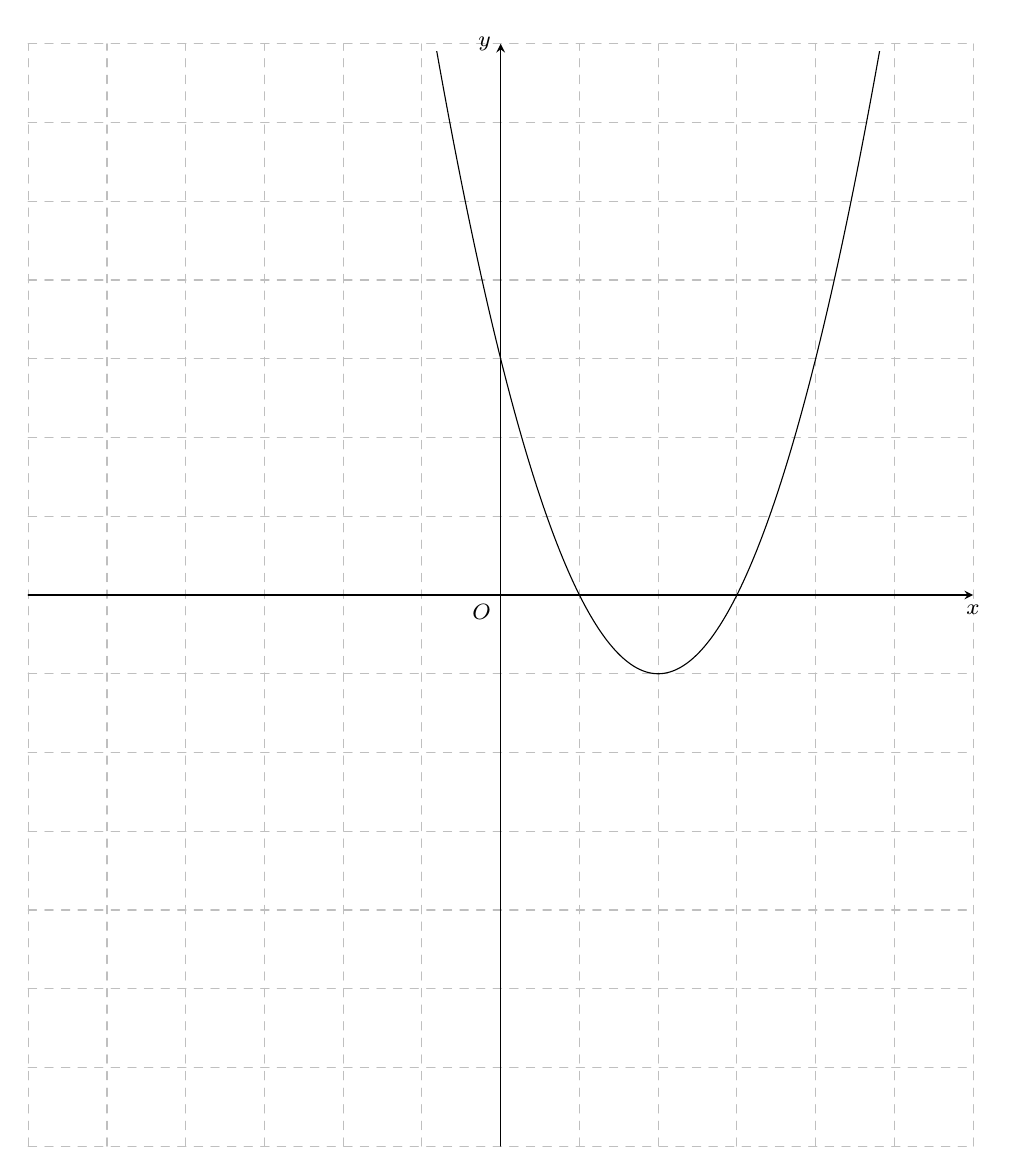
\begin{tikzpicture}[scale=1,>=stealth, font=\footnotesize, line join=round, line cap=round]
	\def\a{1} \def\b{-4} \def\c{3} % Hệ số
	\def\xmin{-6} \def\xmax{6}
	\def\ymin{-7} \def\ymax{7}
	
	\draw[color=gray!50,dashed] (\xmin,\ymin) grid (\xmax,\ymax);
	
	\draw[->] (\xmin,0)--(\xmax,0) node [below]{$x$};
	\draw[->] (0,\ymin)--(0,\ymax) node [left]{$y$};
	\node at (0,0) [below left]{$O$};
	\clip (\xmin+0.1,\ymin+0.1) rectangle (\xmax-0.5,\ymax-0.1);
	\draw[smooth,samples=300] plot(\x,{\a*(\x)^2+\b*(\x)+\c});
\end{tikzpicture}

% Hàm số bậc 3  
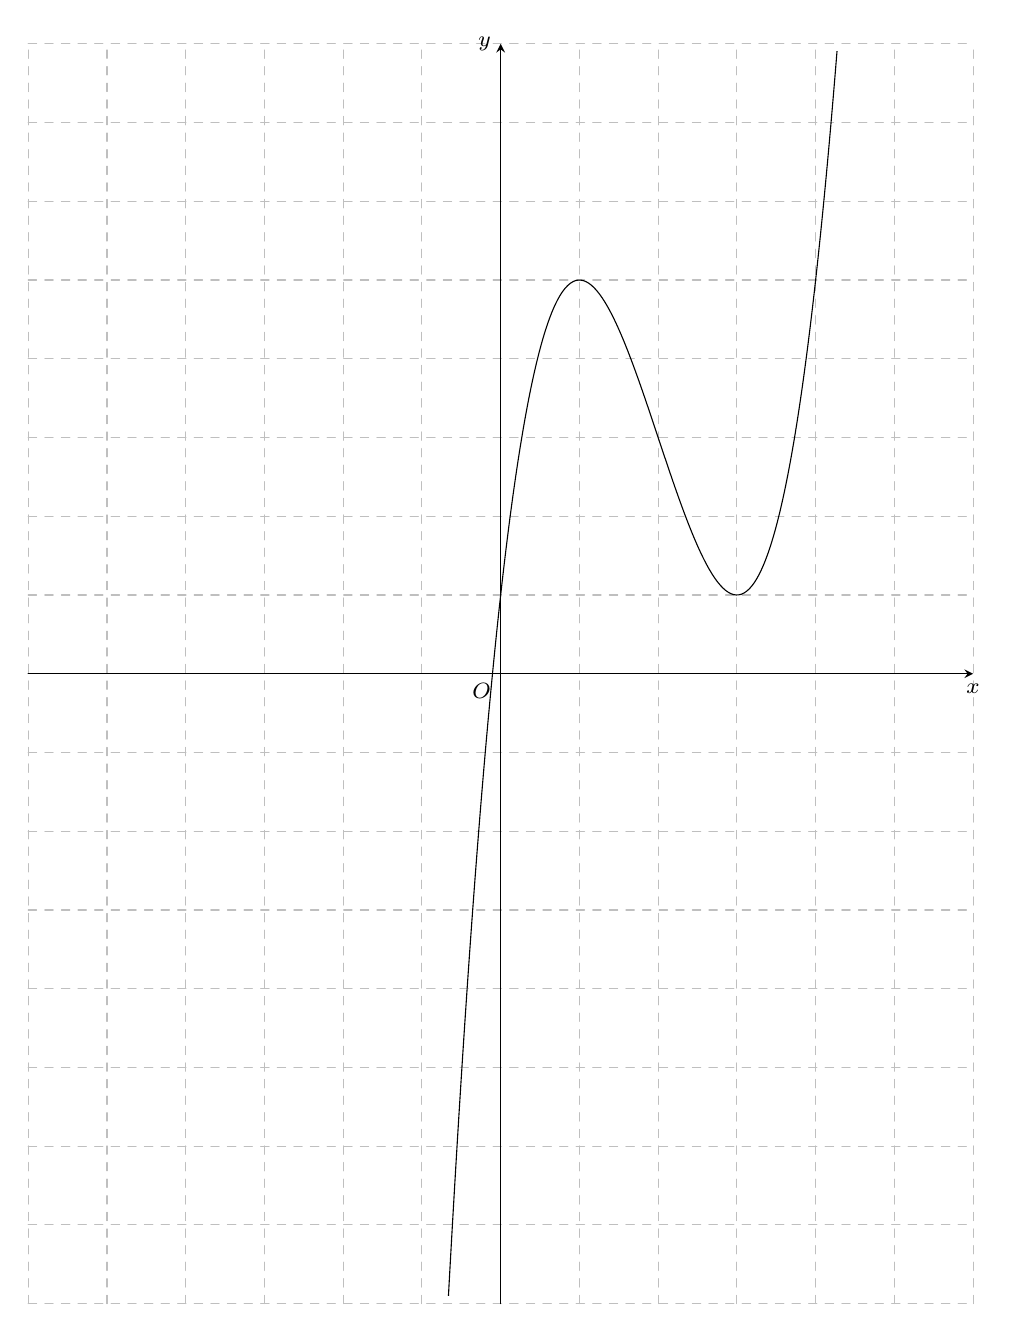
\begin{tikzpicture}[scale=1,>=stealth, font=\footnotesize, line join=round, line cap=round]
	\def\a{1} \def\b{-6} \def\c{9} \def\d{1} % Hệ số
	\def\xmin{-6} \def\xmax{6}
	\def\ymin{-8} \def\ymax{8} 
	\draw[color=gray!50,dashed] (\xmin,\ymin) grid (\xmax,\ymax); 
	\draw[->] (\xmin,0)--(\xmax,0) node [below]{$x$};
	\draw[->] (0,\ymin)--(0,\ymax) node [left]{$y$};
	\node at (0,0) [below left]{$O$};
	\clip (\xmin+0.1,\ymin+0.1) rectangle (\xmax-0.5,\ymax-0.1);
	\draw[smooth,samples=300] plot(\x,{\a*(\x)^3+\b*(\x)^2+\c*(\x)+\d});
\end{tikzpicture}

% Hám số trùng phương 
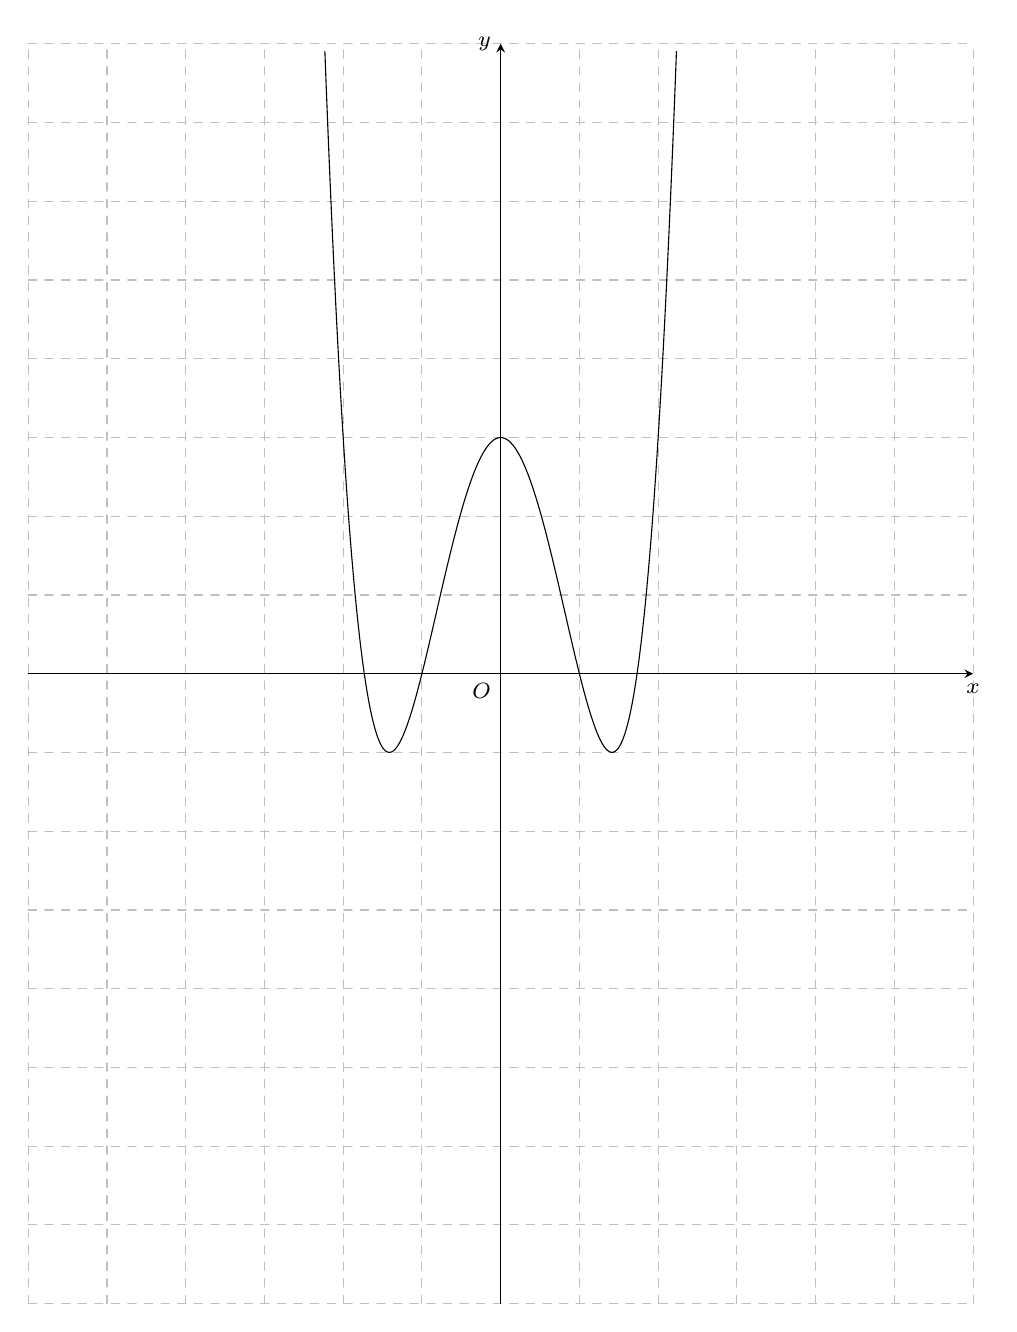
\begin{tikzpicture}[scale=1,>=stealth, font=\footnotesize, line join=round, line cap=round]
	\def\a{1} \def\b{-4} \def\c{3} % Hệ số
	\def\xmin{-6} \def\xmax{6}
	\def\ymin{-8} \def\ymax{8} 
	\draw[color=gray!50,dashed] (\xmin,\ymin) grid (\xmax,\ymax); 
	\draw[->] (\xmin,0)--(\xmax,0) node [below]{$x$};
	\draw[->] (0,\ymin)--(0,\ymax) node [left]{$y$};
	\node at (0,0) [below left]{$O$};
	\clip (\xmin+0.1,\ymin+0.1) rectangle (\xmax-0.5,\ymax-0.1);
	\draw[smooth,samples=300] plot(\x,{\a*(\x)^4+\b*(\x)^2+\c});
\end{tikzpicture}

% Hàm số nhất biến 
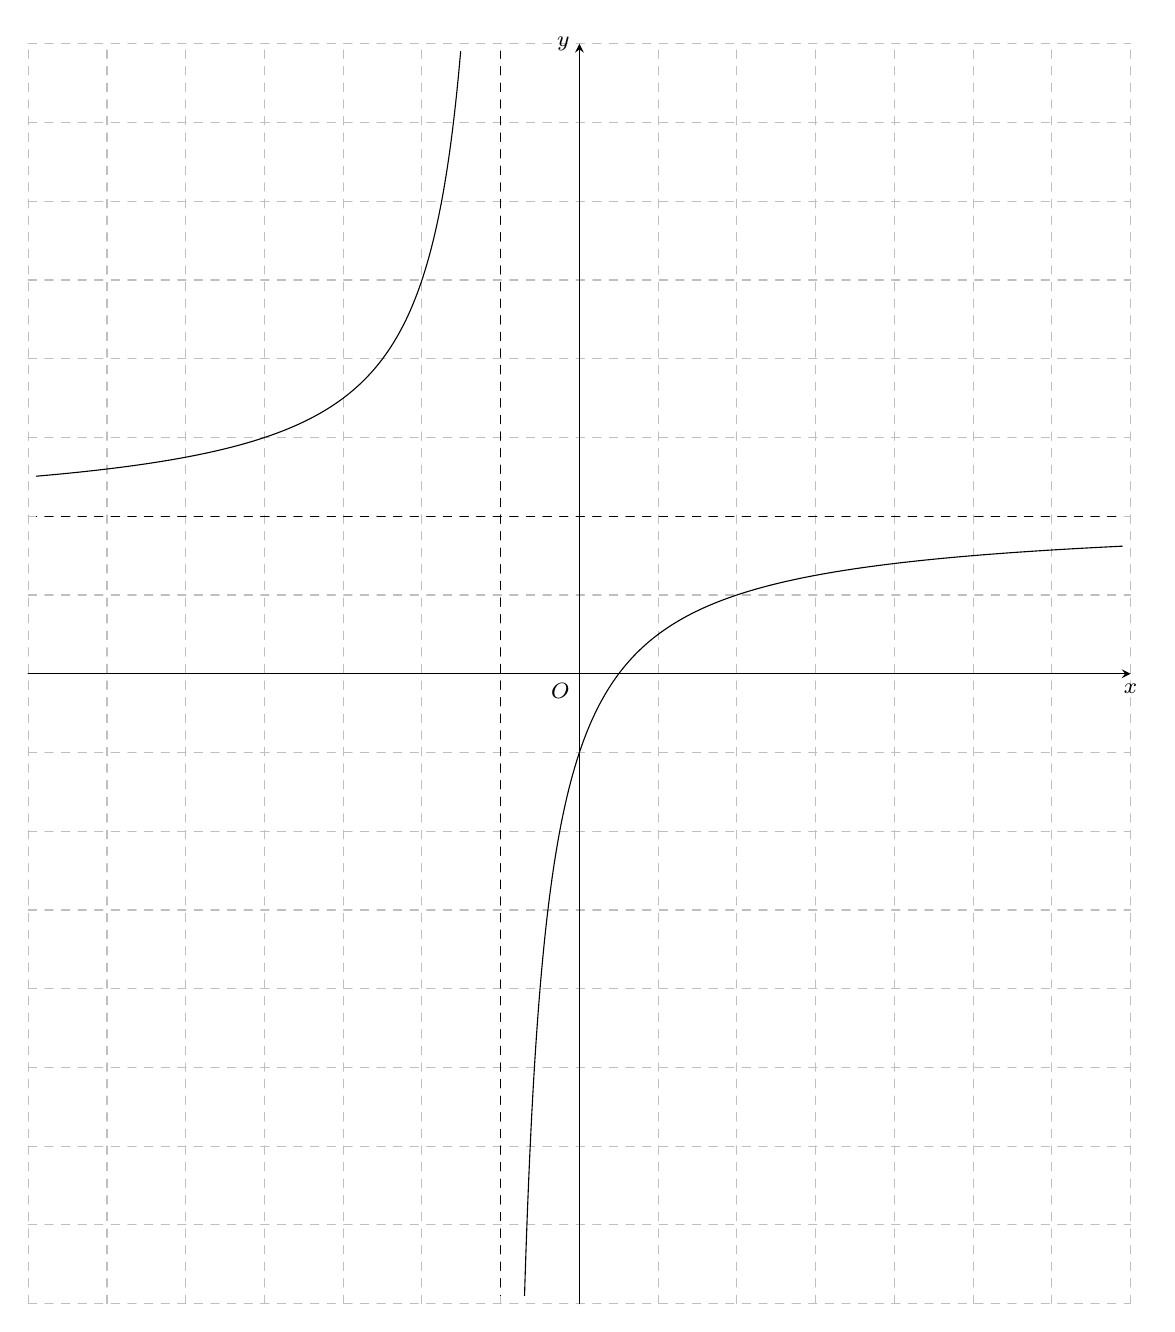
\begin{tikzpicture}[scale=1,>=stealth, font=\footnotesize, line join=round, line cap=round]
	\def\a{2} \def\b{-1} \def\c{1} \def\d{1} % Hệ số
	\def\xmin{-7} \def\xmax{7}
	\def\ymin{-8} \def\ymax{8}
	\draw[color=gray!50,dashed] (\xmin,\ymin) grid (\xmax,\ymax);
	\draw[->] (\xmin,0)--(\xmax,0) node [below]{$x$};
	\draw[->] (0,\ymin)--(0,\ymax) node [left]{$y$};
	\node at (0,0) [below left]{$O$};
	\clip (\xmin+0.1,\ymin+0.1) rectangle (\xmax-0.1,\ymax-0.1);
	\draw[smooth,samples=300,domain=\xmin:(-\d/\c-0.1)] plot(\x,{(\a*(\x)+\b)/(\c*(\x)+\d)});
	\draw[smooth,samples=300,domain=(-\d/\c+0.1:\xmax)] plot(\x,{(\a*(\x)+\b)/(\c*(\x)+\d)});
	\draw[dashed] (-\d/\c,\ymin)--(-\d/\c,\ymax);
	\draw[dashed] (\xmin,\a/\c)--(\xmax,\a/\c);
\end{tikzpicture}

% Hàm số sin 
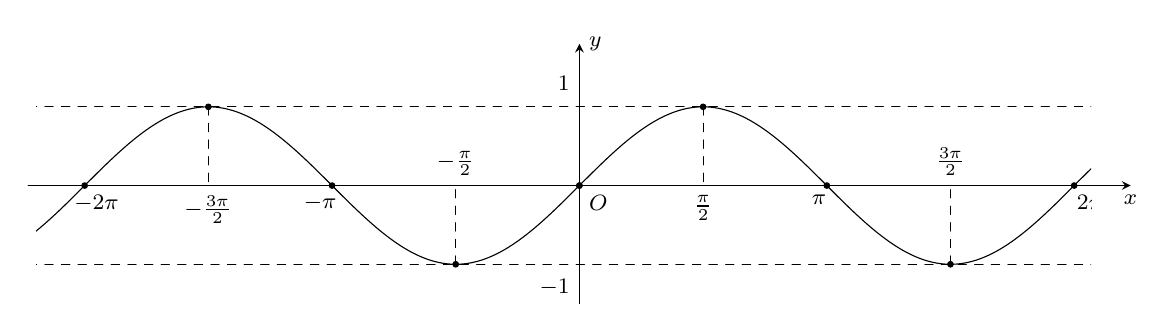
\begin{tikzpicture}[scale=1,>=stealth, font=\footnotesize, line join=round, line cap=round]
	\def\xmin{-7} \def\xmax{7} \def\ymin{-1.5} \def\ymax{1.8}
	\draw[->] (\xmin,0)--(\xmax,0) node [below]{$x$};
	\draw[->] (0,\ymin)--(0,\ymax) node [right]{$y$};
	\node at (0,0) [below right]{$O$};
	\clip (\xmin+0.1,\ymin+0.1) rectangle (\xmax-0.5,\ymax-0.1);
	\draw[smooth,samples=400,domain=\xmin:\xmax] plot(\x,{sin(\x r)});
	\draw[dashed] (\xmin,1)--(\xmax,1) (\xmin,-1)--(\xmax,-1);
	\foreach \x in {-2*pi,-1.5*pi,-pi,-0.5*pi,0}
	{\draw[fill=black] (\x,sin \x*180/pi) circle (1pt);
		\draw[dashed] (\x,sin \x*180/pi)--(\x,0);
		\draw[fill=black] (-\x,sin -\x*180/pi) circle (1pt);
		\draw[dashed] (-\x,sin -\x*180/pi)--(-\x,0);}
	\node at (0,1.3) [left]{$1$};
	\node at (0,-1.3) [left]{$-1$};
	\node at (-2*pi+0.15,0) [below]{$-2\pi$};
	\node at (-1.5*pi,0) [below]{$-\frac{3\pi}{2}$};
	\node at (-pi-0.15,0) [below]{$-\pi$};
	\node at (-0.5*pi,0) [above]{$-\frac{\pi}{2}$};
	\node at (0.5*pi,0) [below]{$\frac{\pi}{2}$};
	\node at (pi-0.1,0) [below]{$\pi$};
	\node at (1.5*pi,0) [above]{$\frac{3\pi}{2}$};
	\node at (2*pi+0.2,0) [below]{$2\pi$};
\end{tikzpicture}

% Hàm số côsin 
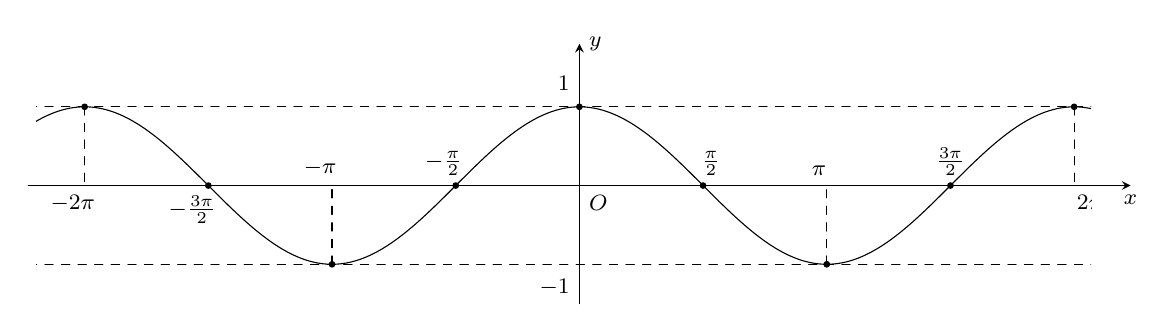
\begin{tikzpicture}[scale=1,>=stealth, font=\footnotesize, line join=round, line cap=round]
	\def\xmin{-7} \def\xmax{7} \def\ymin{-1.5} \def\ymax{1.8}
	\draw[->] (\xmin,0)--(\xmax,0) node [below]{$x$};
	\draw[->] (0,\ymin)--(0,\ymax) node [right]{$y$};
	\node at (0,0) [below right]{$O$};
	\clip (\xmin+0.1,\ymin+0.1) rectangle (\xmax-0.5,\ymax-0.1);
	\draw[smooth,samples=400,domain=\xmin:\xmax] plot(\x,{cos(\x r)});
	\draw[dashed] (\xmin,1)--(\xmax,1) (\xmin,-1)--(\xmax,-1);
	\foreach \x in {-2*pi,-1.5*pi,-pi,-0.5*pi,0}
	{\draw[fill=black] (\x,cos \x*180/pi) circle (1pt);
		\draw[dashed] (\x,cos \x*180/pi)--(\x,0);
		\draw[fill=black] (-\x,cos -\x*180/pi) circle (1pt);
		\draw[dashed] (-\x,cos \x*180/pi)--(-\x,0);}
	\node at (0,1.3) [left]{$1$};
	\node at (0,-1.3) [left]{$-1$};
	\node at (-2*pi-0.15,0) [below]{$-2\pi$};
	\node at (-1.5*pi-0.2,0) [below]{$-\frac{3\pi}{2}$};
	\node at (-pi-0.15,0) [above]{$-\pi$};
	\node at (-0.5*pi-0.15,0) [above]{$-\frac{\pi}{2}$};
	\node at (0.5*pi+0.1,0) [above]{$\frac{\pi}{2}$};
	\node at (pi-0.1,0) [above]{$\pi$};
	\node at (1.5*pi,0) [above]{$\frac{3\pi}{2}$};
	\node at (2*pi+0.2,0) [below]{$2\pi$};
\end{tikzpicture}

% Hàm số tan 
\begin{tikzpicture}[scale=1,>=stealth, font=\footnotesize, line join=round, line cap=round]
	\def\xmin{-7} \def\xmax{7} \def\ymin{-4} \def\ymax{4}
	\draw[->] (\xmin,0)--(\xmax,0) node [below]{$x$};
	\draw[->] (0,\ymin)--(0,\ymax) node [right]{$y$};
	\node at (0,0) [below right]{$O$};
	\clip (\xmin+0.1,\ymin+0.1) rectangle (\xmax-0.5,\ymax-0.1);
	\draw[smooth,samples=400,domain=\xmin:\xmax] plot(\x,{tan(\x r)});
	\node at (-2*pi-0.2,0) [above]{$-2\pi$};
	\node at (-1.5*pi-0.4,0) [below]{$-\frac{3\pi}{2}$};
	\node at (-pi-0.2,0) [above]{$-\pi$};
	\node at (-0.5*pi-0.4,0) [below]{$-\frac{\pi}{2}$};
	\node at (0.5*pi-0.2,0) [below]{$\frac{\pi}{2}$};
	\node at (pi-0.1,0) [above]{$\pi$};
	\node at (1.5*pi-0.3,0) [below]{$\frac{3\pi}{2}$};
	\node at (2*pi+0.2,0) [below]{$2\pi$};
\end{tikzpicture}

% Hàm số Cotan 
\begin{tikzpicture}[scale=1,>=stealth, font=\footnotesize, line join=round, line cap=round]
	\def\xmin{-7} \def\xmax{7} \def\ymin{-4} \def\ymax{4}
	\draw[->] (\xmin,0)--(\xmax,0) node [below]{$x$};
	\draw[->] (0,\ymin)--(0,\ymax) node [left]{$y$};
	\node at (0,0) [above left]{$O$};
	\clip (\xmin+0.1,\ymin+0.1) rectangle (\xmax-0.5,\ymax-0.1);
	\foreach \n in {-2,-1,0,1}
	{\draw[smooth,samples=400,domain=(\n+0.05)*pi:(\n+0.95)*pi] plot(\x,{1/tan(\x r)});
		\draw (\n*pi,\ymin)--(\n*pi,\ymax);}
	\node at (-2*pi-0.4,0) [below]{$-2\pi$};
	\node at (-1.5*pi-0.3,0) [below]{$-\frac{3\pi}{2}$};
	\node at (-pi-0.3,0) [below]{$-\pi$};
	\node at (-0.5*pi-0.3,0) [below]{$-\frac{\pi}{2}$};
	\node at (0.5*pi-0.1,0) [below]{$\frac{\pi}{2}$};
	\node at (pi-0.2,0) [below]{$\pi$};
	\node at (1.5*pi-0.2,0) [below]{$\frac{3\pi}{2}$};
\end{tikzpicture}

% Hàm số lũy thừa 
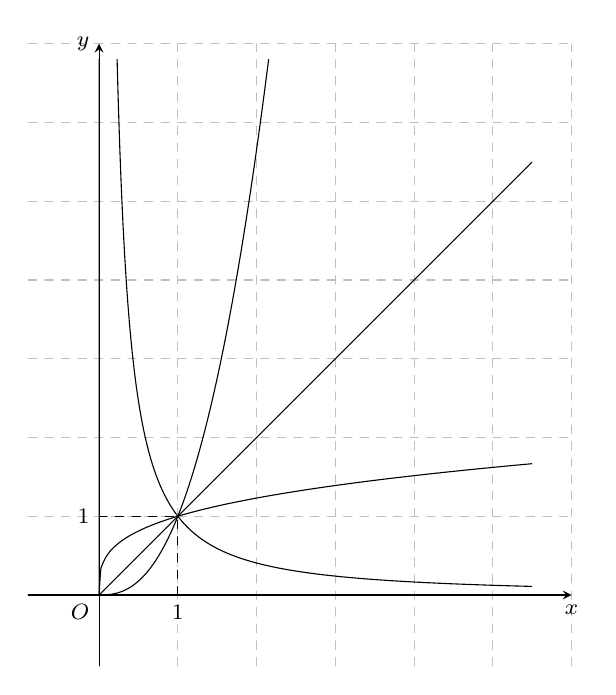
\begin{tikzpicture}[scale=1,>=stealth, font=\footnotesize, line join=round, line cap=round]
	\def\xmax{6} \def\ymax{7}
	\draw[color=gray!50,dashed] (-0.9,-0.9) grid (\xmax,\ymax);
	\draw[->] (-0.9,0)--(\xmax,0) node [below]{$x$};
	\draw[->] (0,-0.9)--(0,\ymax) node [left]{$y$};
	\node at (0,0) [below left]{$O$};
	\clip (-0.9,-0.9) rectangle (\xmax-0.5,\ymax-0.2);
	\draw[smooth,samples=300,domain=0:\xmax] plot(\x,{(\x)^2.5});
	\draw[smooth,samples=300,domain=0:\xmax] plot(\x,{\x});
	\draw[smooth,samples=300,domain=0:\xmax] plot(\x,{(\x)^0.3});
	\draw[smooth,samples=300,domain=0:\xmax] plot(\x,{(\x)^(-1.3)});
	\draw[dashed] (1,0) node[below]{$1$}--(1,1)--(0,1)node[left]{$1$};
\end{tikzpicture}

% Hàm số mũ 
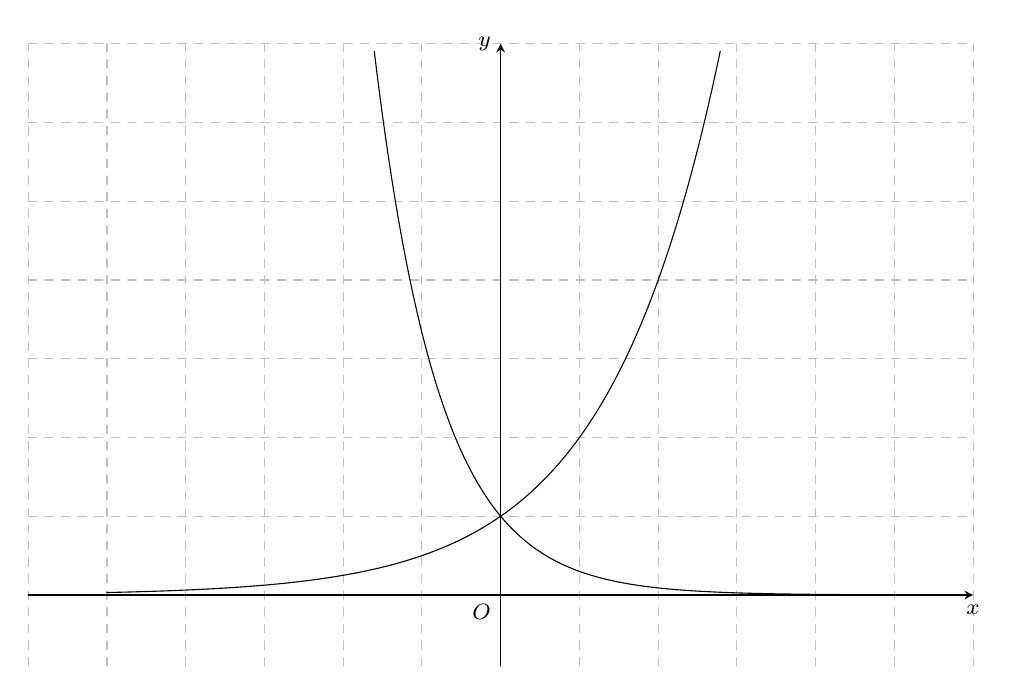
\begin{tikzpicture}[scale=1,>=stealth, font=\footnotesize, line join=round, line cap=round]
	\def\xmin{-6} \def\xmax{6} \def\ymax{7}
	\draw[color=gray!50,dashed] (\xmin,-0.9) grid (\xmax,\ymax);
	\draw[->] (\xmin,0)--(\xmax,0) node [below]{$x$};
	\draw[->] (0,-0.9)--(0,\ymax) node [left]{$y$};
	\node at (0,0) [below left]{$O$};
	\clip (\xmin,-0.9) rectangle (\xmax-0.1,\ymax-0.1);
	\draw[smooth,samples=300] plot(\x,{2^(\x)});
	\draw[smooth,samples=300] plot(\x,{0.3^(\x)});
\end{tikzpicture}

% Hàm số lôgarit 
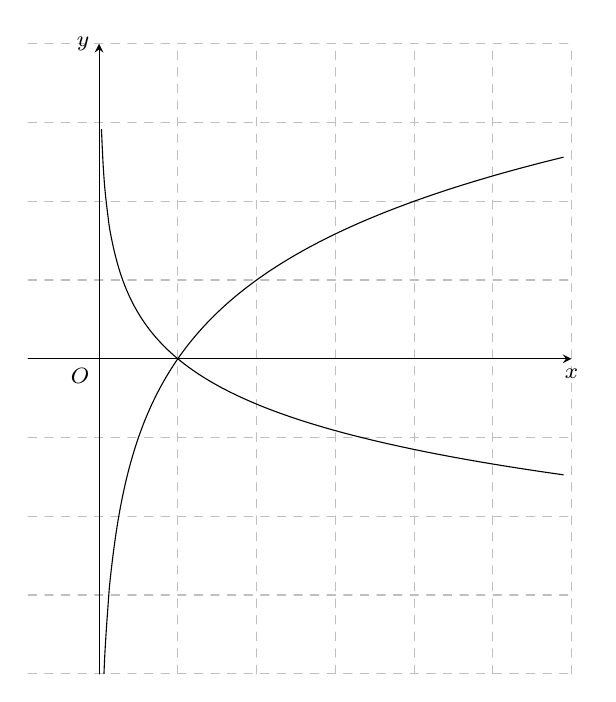
\begin{tikzpicture}[scale=1,>=stealth, font=\footnotesize, line join=round, line cap=round]
	\def\xmax{6} \def\ymin{-4} \def\ymax{4}
	\draw[color=gray!50,dashed] (-0.9,\ymin) grid (\xmax,\ymax);
	\draw[->] (-0.9,0)--(\xmax,0) node [below]{$x$};
	\draw[->] (0,\ymin)--(0,\ymax) node [left]{$y$};
	\node at (0,0) [below left]{$O$};
	\clip (-0.9,\ymin) rectangle (\xmax-0.1,\ymax-0.1);
	\draw[smooth,samples=300,domain=0.03:\xmax] plot(\x,{ln(\x)/ln(2)});
	\draw[smooth,samples=300,domain=0.03:\xmax] plot(\x,{ln(\x)/ln(0.3)});
\end{tikzpicture}

% Hệ trục cơ bản 
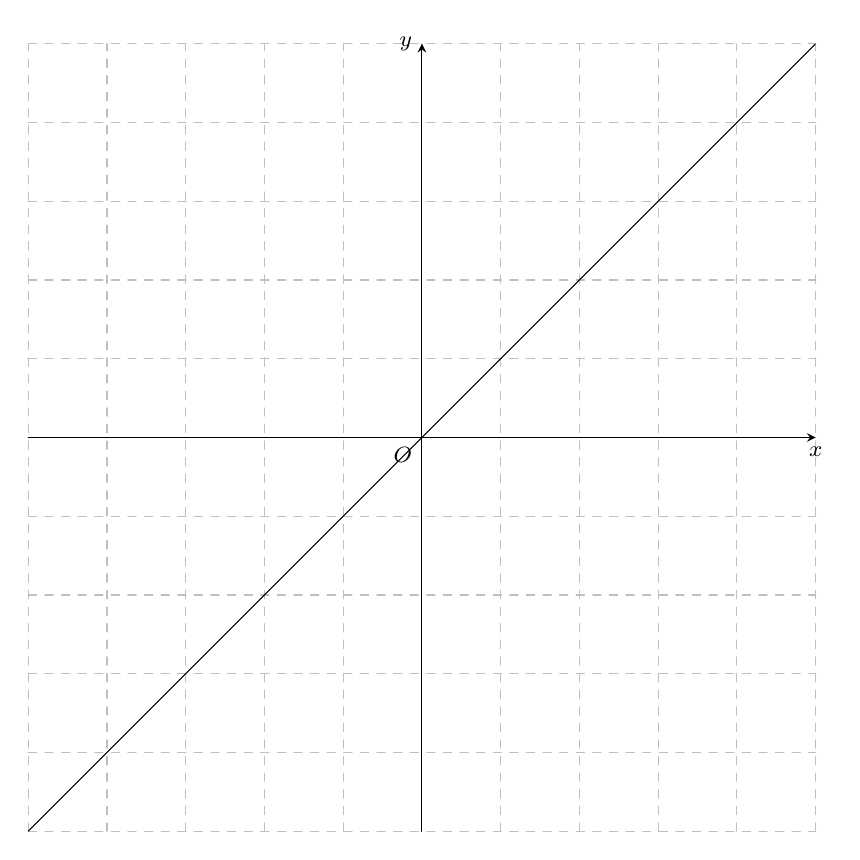
\begin{tikzpicture}[scale=1,>=stealth, font=\footnotesize, line join=round, line cap=round]
	\draw[color=gray!50,dashed] (-5,-5) grid (5,5);
	\draw[->] (-5,0)--(5,0) node [below]{$x$};
	\draw[->] (0,-5)--(0,5) node [left]{$y$};
	\node at (0,0) [below left]{$O$};
	\clip (-5,-5) rectangle (5,5);
	\draw[smooth,samples=300] plot(\x,{\x});
\end{tikzpicture}

% Ghi số lên trục 
\foreach \x in {-3,-2,...,3}
\draw[thin] (\x,1pt)--(\x,-1pt) node [below] {$\x$};
\foreach \y in {-3,-2,...,3}
\draw[thin] (1pt,\y)--(-1pt,\y) node [left] {$\y$};

% Bảng biến thiên, bảng xét dấu 

% Bậc 3 - 1 cực đại, 1 cực tiểu 
\begin{center}
	
\begin{tikzpicture}
		\tkzTabInit[nocadre=false,lgt=1.2,espcl=2.5,deltacl=0.6]
		{$x$ /0.6, $y'$ /0.6, $y$ /2.5}
		{$-\infty$,$x_1$,$x_2$,$+\infty$}
		\tkzTabLine{,+,$0$,-,$0$,+,}
		\tkzTabVar{-/$-\infty$,+/$y_1$,-/$y_2$,+/$+\infty$}
	\end{tikzpicture}
\end{center}

% Bậc 3 - y' giải 1 nghiệm 
\begin{center}
	
\begin{tikzpicture}
		\tkzTabInit[nocadre=false,lgt=1.2,espcl=2.5,deltacl=0.6]
		{$x$/0.6,$y'$/0.6,$y$/2}
		{$-\infty$,,$+\infty$}
		\tkzTabLine{,+,$0$,+,}
		\tkzTabVar{-/$-\infty$,R,+/$+\infty$}
		\tkzTabVal{1}{3}{0.5}{$x_0$}{$y_0$}
	\end{tikzpicture}
\end{center}

% Bậc 3 - y' giải vô nghiệm 
\begin{center}
	
\begin{tikzpicture}
		\tkzTabInit[nocadre=false,lgt=1.2,espcl=2.5,deltacl=0.6]
		{$x$/0.6,$y'$/0.6,$y$/2}
		{$-\infty$,$+\infty$}
		\tkzTabLine{,-,}
		\tkzTabVar{+/$+\infty$,-/$-\infty$}
	\end{tikzpicture}
\end{center}

% Trùng phương - có 3 cực trị 
\begin{center}
	
\begin{tikzpicture}
		\tkzTabInit[nocadre=false,lgt=1.2,espcl=2.5,deltacl=0.6]
		{$x$ /0.6,$y'$ /0.6,$y$ /2}
		{$-\infty$,$x_1$,$0$,$x_3$,$+\infty$}
		\tkzTabLine{,+,$0$,-,$0$,+,$0$,-,}
		\tkzTabVar{-/$-\infty$, +/$y_1$,-/$y_2$,+/$y_3$,-/$-\infty$}
	\end{tikzpicture}
\end{center}

% Trùng phương có 1 cực trị 
\begin{center}
	
\begin{tikzpicture}
		\tkzTabInit[nocadre=false,lgt=1.2,espcl=2.5,deltacl=0.6]
		{$x$ /0.6,$y'$ /0.6,$y$ /2}
		{$-\infty$,$0$,$+\infty$}
		\tkzTabLine{,+,$0$,-,}
		\tkzTabVar{-/$-\infty$, +/$y_0$,-/$-\infty$}
	\end{tikzpicture}
\end{center}

% Hàm số Nhất biến 
\begin{center}
	
\begin{tikzpicture}
		\tikzset{double style/.append style={double distance=1.5pt}}
		\tkzTabInit[nocadre=false,lgt=1.2,espcl=2.5,deltacl=0.6]
		{$x$ /0.6,$y'$ /0.6,$y$ /2}
		{$-\infty$,$x_0$,$+\infty$}
		\tkzTabLine{,+,d,+,}
		\tkzTabVar{-/$y_0$,+D-/$+\infty$/$-\infty$,+/$y_0$}
	\end{tikzpicture}
\end{center}

% Bậc 2 trên bậc 1 - có 2 cực trị 
\begin{center}
	
\begin{tikzpicture}
		\tikzset{double style/.append style={double distance=1.5pt}}
		\tkzTabInit[nocadre=false,lgt=1.2,espcl=2.5,deltacl=0.6]
		{$x$ /0.6,$y'$ /0.6,$y$ /2}
		{$-\infty$,$x_1$,$x_0$,$x_2$,$+\infty$}
		\tkzTabLine{,+,$0$,-,d,-,$0$,+,}
		\tkzTabVar{-/$-\infty$,+/$y_1$,-D+/$-\infty$/$+\infty$,-/$y_2$,+/$+\infty$}
	\end{tikzpicture}
\end{center}

% Thủ thuật chống tràn ô 
\tkzTabInit[nocadre=false,lgt=1.2,espcl=2.5,deltacl=1]

% Thủ thuật tăng |..|
\tikzset{double style/.append style={double distance=1.5pt}}

% Thủ thuật thêm giá trị số 1 - Chèn x_0,y_0 vào giữa cột 1 & 2
\tkzTabVal[draw]{1}{2}{0.5}{$x_0$}{$y_0$}

% Thủ thuật thêm giá trị số 2 - 
\begin{center}
	\begin{tikzpicture}[>=stealth,scale=1]
		\tkzTabInit[lgt=1.2,espcl=2.5]
		{$x$ /.6, $f'(x)$ /0.6, $f(x)$ /2.6}
		{$-\infty$,$1$,$4$,$+\infty$}
		\tkzTabLine{,+,$0$,-,$0$,-,}
		\tkzTabVar{-/$-\infty$,+/$3$,R,-/$-5$}
		\path (FR22) -- (FL42)node[midway,fill=white](M){$-4$};
		\draw[arrow style,shorten >=-2pt](FR22)--(M);
	\end{tikzpicture}
\end{center}

% Thủ thuật xóa khoảng số 1 
\begin{tikzpicture}\tkzTabInit[nocadre=false,lgt=1.2,espcl=2.5,deltacl=0.6]
	{$x$/0.6,$y$/3}
	{,$x_I$,$0$,$2$,}
	\fill[pattern color=green!50,pattern=dots] (T11) rectangle (N32) (N41) rectangle (T22);
	\draw (T11) rectangle (N32) (N41) rectangle (T22);
	\tkzTabVar{+/,-/,R,R,+/}
\end{tikzpicture}

% Thủ thuật xóa khoảng số 2 
\begin{center}
	
\begin{tikzpicture}
		\tkzTabInit[nocadre=false,lgt=1.2,espcl=2.5,deltacl=0.6]
		{$x$/0.6,$f’(x)$/0.6,$f(x)$/2.5}
		{$-\infty$,$a$,$b$,$c$,$+\infty$}
		\tkzTabLine{,-,d,h,d,-,z,+,}
		\tkzTabVar{+/$+\infty$,-DH/$-\infty$,D+/$m$,-/$n$,+/$+\infty$}
	\end{tikzpicture}
\end{center}

% Bảng xét dấu 1 dòng 
\begin{center}
	
\begin{tikzpicture}
		\tkzTabInit[nocadre=false,lgt=2,espcl=2,deltacl=0.6]
		{$x$ /0.6,$x^2+x-2$ /0.6}
		{$-\infty$,$-2$,$1$,$+\infty$}
		\tkzTabLine{,+,$0$,-,$0$,+,}
	\end{tikzpicture}
\end{center}

% Bảng xét dấu 1 dòng có xóa 
\begin{center}
	
\begin{tikzpicture}
		\tkzTabInit[nocadre=false,lgt=1.2,espcl=1.5,deltacl=0.6]
		{$x$ /0.6,$f(x)$ /0.6}
		{$0$,$1$,$2$,$3$}
		\tkzTabLine{z,+,d,h,d,-,t}
	\end{tikzpicture}
\end{center}

% Bảng xét dấu 3 dòng 
\begin{center}
	
\begin{tikzpicture}
		\tkzTabInit[nocadre=false,lgt=2.1,espcl=2,deltacl=0.6]
		{$x$ /0.6,$x^2-x+6$ /0.6,$x-1$ /0.6,$\dfrac{x^2-x-6}{x-1}$ /1.1}
		{$-\infty$,$-2$,$1$,$3$,$+\infty$}
		\tkzTabLine{,+,$0$,-,|,-,$0$,+,}
		\tkzTabLine{,-,|,-,$0$,+,|,+,}
		\tkzTabLine{,-,$0$,+,||,-,$0$,+,}
	\end{tikzpicture}
\end{center}

% % Trục số 
% Khởi tạo 

\begin{tikzpicture}[>=stealth,line width=1pt,color=red]
	\draw[->](-3,0)->(11,0);		%Vẽ trục số
	\def\skipInterval{0.5cm}		%Khoảng cách đặt nhãn
	\def\colorInterval{blue} 	%Màu tick, màu fill miền
	
\end{tikzpicture}

% Gạch phải qua trái - không fill miền 
\IntervalR{\big(}{2}{\big]}{5}

% Gạch trái qua phải - không fill miền
\IntervalL{\big[}{-2}{\big)}{1}

% Gạch phải qua trái - fill miền 
\IntervalRF{\big(}{2}{\big]}{5}

% Gạch trái qua phải - fill miền 
\IntervalLF{\big[}{-2}{\big)}{1}

% Gạch đứng  
\Interval{\big(}{7}{\big]}{9}

% Gạch trái qua phải fill miền với nhãn tùy ý
\IntervalLR{-3}{-1.4}		\IntervalGLF{}{}{\big)}{-\sqrt{2}}

% Gạch phải qua trái fill miền với nhãn tùy ý
\IntervalLR{2.71}{6.28}		\IntervalGRF{\big(}{e}{\big)}{\pi}

% %Thầy Trần Anh Tuấn
Cần khai báo gói tikz và gói ex_test
%Cấu trúc lệnh
\Interval{tham số 1}{tham số 2}{tham số 3}{tham số 4}
chẳng hạn, biểu diễn (1;3] thì dùng lệnh \Interval{(}{1}{]}{3}
Thêm các chữ cái:
L: Gạch trái qua phải.
R: Gạch phải qua trái.
F: Fill miền.
G: Tổng quát.
Có thể kết hợp các chữ cái.






